\section{Introduction}
The following document contains the Test Specifications for our system. Testing is crucial and it ensures that the system, at the end of the project and each Sprint, meets the acceptance criteria specified. In Scrum testing is done continuously in every Sprint. \\
\\
At the end of all Sprints we shall be able to deliver a Potentially Shippable Product based on the Sprint Backlog. This is fundamental because when work is divided into simple pieces it can be be finished in a short period of time. Before we can address a part of our system as a Potentially Shippable Product each User Story from the Sprint Backlog needs to be tested. To be able to verify a User Story, we determine specific Acceptance Criteria. These are formulated based on the Agile GIVEN, WHEN and THEN-method, also called Gherkin. This method makes it easy to test small parts of the system. The tests done based on the Acceptance Criteria are often called Unit Tests.\\
\\
There will be performed a set of verification tests in each Sprint relating to the User Story as mention above. Verification tests helps us verify that we have developed the the right solution based on the Acceptance Criteria stated. \cite{ref1}\\
\\
The template presented in Fig. \ref{fig:testtemp} functions as a verification record where our Acceptance Criteria are tested. Each test card states an unique test ID, which Acceptance Criteria, Backlog Item and Jira ID it relates to and in which Sprint the verification test was done. It also  displays which Verification Procedure we will use and the results of the test.\\
\begin{figure}[h]
    \centering
        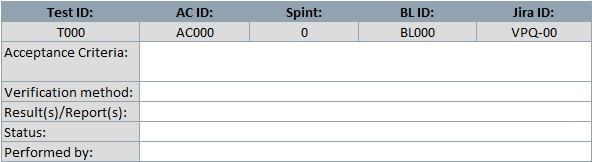
\includegraphics[width=0.9\textwidth]{VAPIQ-PICTURES/testtemp}
        \caption{Verification Test Card Template}
        \label{fig:testtemp}
\end{figure}
\\
Many Verification Tests in Scrum are easily executed, but some tests are more extensive and needs a more detailed procedure and elaborative result. In these situations a Test Report is generated. These will be referred to in the Result(s)/Report(s) tab as  Fig. \ref{fig:testtemp}. Verification Tests determines whether or not the Acceptance Criteria are fulfilled through for example inspection, calculation and measurements.\\ 
\\
In Fig. \ref{fig:testsetup} we see a simple illustration of how the Verification Test process works. 
\begin{figure}[h]
    \centering
        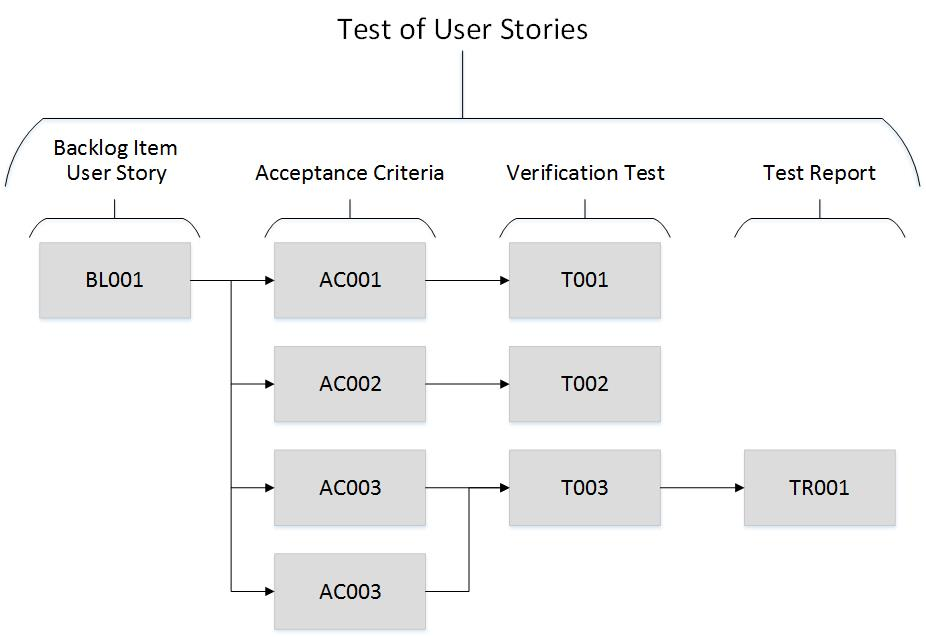
\includegraphics[width=0.9\textwidth]{VAPIQ-PICTURES/testdocbild}
        \caption{Test of User Stories}
        \label{fig:testsetup}
\end{figure}